%
% File naaclhlt2015.tex
%

\documentclass[11pt,letterpaper]{article}
\usepackage{naaclhlt2015}
\usepackage{times}
\usepackage{latexsym}
\usepackage[cmex10]{amsmath}
\usepackage{xspace}
\usepackage{url}
\usepackage{subcaption}
\usepackage{graphicx}
\usepackage{float}
\usepackage{tikz}
\usetikzlibrary{fit,positioning}

% macros of Wei-Lwun
% =============================================================================
% New commands
% -----------------------------------------------------------------------------


\newcommand{\eg}{\emph{e.g.}\@\xspace}
\newcommand{\ie}{\emph{i.e.}\@\xspace}

\makeatletter
\newcommand{\etc}{%
    \@ifnextchar{.}%
        {\emph{etc}}%
        {\emph{etc.}\@\xspace}%
}
\newcommand{\etal}{%
    \@ifnextchar{.}%
        {\emph{et al}}%
        {\emph{et al.}\@\xspace}%
}
\makeatother


\newcommand{\vect}[1]{\boldsymbol{#1}}
\newcommand{\argmax}[1]{\underset{#1}{arg\,max}\,\,}
\newcommand{\argmin}[1]{\underset{#1}{arg\,min}\,\,}
\newcommand{\expect}[1]{\langle #1 \rangle}
\newcommand{\normone}[1]{\| #1 \|_1}
\newcommand{\meanvar}[2]{#1\,{\scriptsize (#2)}}
\newcommand{\bigspace}[0]{\;\;\;\;\;\;\;\;\;\;\;\;\;\;\;\;\;\;\;\;\;\;\;\;\;\;\;\;\;\;\;\;\;\;\;\;\,}
\newcommand{\naive}{na\"ive }
\newcommand{\refeq}[1]{Eq.~(\ref{#1})}
\newcommand{\reffig}[1]{Figure \ref{#1}}
\newcommand{\what}[1]{\widehat{#1}}


% Mathmatics (from Kevin Murphy)
\newcommand{\be}{\begin{equation}}
\newcommand{\ee}{\end{equation}}

\newcommand{\myvec}[1]{\mbox{$\mathbf{#1}$}}
\newcommand{\myvecsym}[1]{\mbox{$\boldsymbol{#1}$}}

\newcommand{\vzero}{\mbox{$\myvecsym{0}$}}
\newcommand{\vone}{\mbox{$\myvecsym{1}$}}

\newcommand{\valpha}{\mbox{$\myvecsym{\alpha}$}}
\newcommand{\vbeta}{\mbox{$\myvecsym{\beta}$}}
\newcommand{\vdelta}{\mbox{$\myvecsym{\delta}$}}
\newcommand{\vepsilon}{\mbox{$\myvecsym{\epsilon}$}}
\newcommand{\veta}{\mbox{$\myvecsym{\eta}$}}
\newcommand{\vgamma}{\mbox{$\myvecsym{\gamma}$}}
\newcommand{\vmu}{\mbox{$\myvecsym{\mu}$}}
\newcommand{\vlambda}{\mbox{$\myvecsym{\lambda}$}}
\newcommand{\vLambda}{\mbox{$\myvecsym{\Lambda}$}}
\newcommand{\vphi}{\mbox{$\myvecsym{\phi}$}}
\newcommand{\vPhi}{\mbox{$\myvecsym{\Phi}$}}
\newcommand{\vpi}{\mbox{$\myvecsym{\pi}$}}
\newcommand{\vPsi}{\mbox{$\myvecsym{\Psi}$}}
\newcommand{\vtheta}{\mbox{$\myvecsym{\theta}$}}
\newcommand{\vTheta}{\mbox{$\myvecsym{\Theta}$}}
\newcommand{\vsigma}{\mbox{$\myvecsym{\sigma}$}}
\newcommand{\vSigma}{\mbox{$\myvecsym{\Sigma}$}}
\newcommand{\vtau}{\mbox{$\myvecsym{\tau}$}}
\newcommand{\vxi}{\mbox{$\myvecsym{\xi}$}}

\newcommand{\va}{\mbox{$\myvec{a}$}}
\newcommand{\vb}{\mbox{$\myvec{b}$}}
\newcommand{\vc}{\mbox{$\myvec{c}$}}
\newcommand{\vd}{\mbox{$\myvec{d}$}}
\newcommand{\ve}{\mbox{$\myvec{e}$}}
\newcommand{\vf}{\mbox{$\myvec{f}$}}
\newcommand{\vg}{\mbox{$\myvec{g}$}}
\newcommand{\vh}{\mbox{$\myvec{h}$}}
\newcommand{\vj}{\mbox{$\myvec{j}$}}
\newcommand{\vk}{\mbox{$\myvec{k}$}}
\newcommand{\vm}{\mbox{$\myvec{m}$}}
\newcommand{\vn}{\mbox{$\myvec{n}$}}
\newcommand{\vp}{\mbox{$\myvec{p}$}}
\newcommand{\vq}{\mbox{$\myvec{q}$}}
\newcommand{\vr}{\mbox{$\myvec{r}$}}
\newcommand{\vs}{\mbox{$\myvec{s}$}}
\newcommand{\vt}{\mbox{$\myvec{t}$}}
\newcommand{\vu}{\mbox{$\myvec{u}$}}
\newcommand{\vv}{\mbox{$\myvec{v}$}}
\newcommand{\vw}{\mbox{$\myvec{w}$}}
\newcommand{\vx}{\mbox{$\myvec{x}$}}
\newcommand{\vxt}{\mbox{$\myvec{\tilde{x}}$}}
\newcommand{\vy}{\mbox{$\myvec{y}$}}
\newcommand{\vyt}{\mbox{$\myvec{\tilde{y}}$}}
\newcommand{\vz}{\mbox{$\myvec{z}$}}

\newcommand{\vA}{\mbox{$\myvec{A}$}}
\newcommand{\vB}{\mbox{$\myvec{B}$}}
\newcommand{\vC}{\mbox{$\myvec{C}$}}
\newcommand{\vD}{\mbox{$\myvec{D}$}}
\newcommand{\vE}{\mbox{$\myvec{E}$}}
\newcommand{\vF}{\mbox{$\myvec{F}$}}
\newcommand{\vG}{\mbox{$\myvec{G}$}}
\newcommand{\vH}{\mbox{$\myvec{H}$}}
\newcommand{\vI}{\mbox{$\myvec{I}$}}
\newcommand{\vJ}{\mbox{$\myvec{J}$}}
\newcommand{\vK}{\mbox{$\myvec{K}$}}
\newcommand{\vL}{\mbox{$\myvec{L}$}}
\newcommand{\vM}{\mbox{$\myvec{M}$}}
\newcommand{\vN}{\mbox{$\myvec{N}$}}
\newcommand{\vO}{\mbox{$\myvec{O}$}}
\newcommand{\vP}{\mbox{$\myvec{P}$}}
\newcommand{\vQ}{\mbox{$\myvec{Q}$}}
\newcommand{\vR}{\mbox{$\myvec{R}$}}
\newcommand{\vS}{\mbox{$\myvec{S}$}}
\newcommand{\vT}{\mbox{$\myvec{T}$}}
\newcommand{\vU}{\mbox{$\myvec{U}$}}
\newcommand{\vV}{\mbox{$\myvec{V}$}}
\newcommand{\vW}{\mbox{$\myvec{W}$}}
\newcommand{\vX}{\mbox{$\myvec{X}$}}
\newcommand{\vY}{\mbox{$\myvec{Y}$}}
\newcommand{\vZ}{\mbox{$\myvec{Z}$}}

% bar
\newcommand{\vgbar}{\mbox{$\overline{\vg}$}}
\newcommand{\vxbar}{\mbox{$\overline{\vx}$}}
\newcommand{\vybar}{\mbox{$\overline{\vy}$}}
\newcommand{\vzbar}{\mbox{$\overline{\vz}$}}
\newcommand{\vpbar}{\mbox{$\overline{\vp}$}}
\newcommand{\vbbar}{\mbox{$\overline{\vb}$}}

% displacement
\newcommand{\dvc}{\mbox{$\delta\vc$}}

% partial derivative
\newcommand{\pvr}{\mbox{$\partial\vr$}}
\newcommand{\pvc}{\mbox{$\partial\vc$}}

% probability distributions
\newcommand{\betadist}{\mbox{Beta}}
\newcommand{\bernoulli}{\mbox{Ber}}
\newcommand{\Ber}{\mbox{Ber}}
\newcommand{\Binom}{\mbox{Bin}}
\newcommand{\binomdist}{\mbox{Bin}}
\newcommand{\Dir}{\mbox{Dir}}
\newcommand{\discrete}{\mbox{discrete}}
\newcommand{\Discrete}{\mbox{Discrete}}
\newcommand{\expdist}{\mbox{Exp}}
\newcommand{\gammadist}{\mbox{Ga}}
\newcommand{\Ga}{\mbox{Ga}}
\newcommand{\gauss}{\mbox{${\cal N}$}}
\newcommand{\IG}{\mbox{IG}}
\newcommand{\Mu}{\mbox{Mu}}
\newcommand{\Multi}{\mbox{Mu}}
\newcommand{\NIX}{\mbox{$NI\chi^2$}}
\newcommand{\NIG}{\mbox{NIG}}
\newcommand{\NGdist}{\mbox{NG}}
\newcommand{\prob}{\mbox{$p$}}
\newcommand{\Poi}{\mbox{Poi}}
\newcommand{\Student}{\mbox{${\cal T}$}}
\newcommand{\student}{\mbox{${\cal T}$}}
\newcommand{\Wishart}{\mbox{Wi}}
\newcommand{\Wi}{\mbox{Wi}}

% =============================================================================

% =============================================================================
% Renew commands
% -----------------------------------------------------------------------------
\renewcommand{\min}[1]{\underset{#1}{min}\,\,}
\renewcommand{\max}[1]{\underset{#1}{max}\,\,}
% =============================================================================


\interfootnotelinepenalty=10000
\setlength\titlebox{5.0cm}    % Expanding the titlebox 6.5

\title{Relation Extraction from Community Generated Question-Answer Pairs}

\author{
Denis Savenkov\\
Emory University\\ %\Thanks{Research done during an internship at Google}\\
{\tt dsavenk@emory.edu}
\And
Wei-Lwun Lu\\
Google\\
{\tt weilwunlu@google.com}
\AND
Jeff Dalton\\
Google\\
{\tt jeffdalton@google.com}
\And
Eugene Agichtein\\
Emory University\\
{\tt eugene@mathcs.emory.edu}}

\date{}

\begin{document}
\maketitle

\begin{abstract}
\input{abstract.inc}
\end{abstract}

\section{Introduction}
\label{sec:intro}
Traditionally question answering systems used text document collections to retrieve passages relevant to a question and to extract candidate answers \cite{Vrandecic:2014:WFC:2661061.2629489}.
Unfortunately, a paragraph of text encodes a very limited amount of information about answer candidates and predictions has to be used instead, \eg most of the systems estimate candidate answer entity type to match against the expected type inferred from the question text.
On the other hand, modern large scale open-domain knowledge bases, such as dbPedia \cite{auer2007dbpedia}, Freebase \cite{Bollacker:2008:FCC:1376616.1376746} and WikiData \cite{Vrandecic:2014:WFC:2661061.2629489} store a vast amount of general knowledge about different kinds of entities.
This information, encoded as \texttt{[subject, predicate, object]} RDF triples, can be effectively queried using structured query languages, such as SPARQL.
Of course, regular users would rather prefer to ask natural language questions.
Translation of text questions into structured query languages is very challenging for a number of reasons: complexity of a KB schema, variability of natural language and knowledge representation \etc
For example, Figure \ref{fig:example_sparql} gives a SPARQL query that retrieves the answer to a relatively easy question \textit{``who is the current president of the dominican republic in 2010?''}.
% The same information can be asked in many different ways, for example: \textit{``who is the dominican republic president in 2010?''}, or \textit{``who was the leader of the dominican republic in 2010?''} \etc

\begin{figure*}
\centering
\begin{lstlisting}[frame=single]
PREFIX : <http://rdf.freebase.com/ns/>
SELECT DISTINCT ?name {
   :m.027rn :government.governmental_jurisdiction.governing_officials ?gov_position .
   ?gov_position :government.government_position_held.basic_title :m.060c4 .
   ?gov_position :government.government_position_held.office_holder ?president .
   ?gov_position :government.government_position_held.from ?from_date .
   ?gov_position :government.government_position_held.to ?to_date .
   FILTER (
       xsd:date(?from_date) <= "2010"^^xsd:date AND
       xsd:date(?to_date) >= "2010"^^xsd:date
   )
   ?president :type.object.name ?name
}
\end{lstlisting}
\caption{SPARQL query that retrieves the answer to the query \textit{``who is the current president of the dominican republic in 2010?''}}
\label{fig:example_sparql}
\end{figure*}

\begin{figure}
\centering
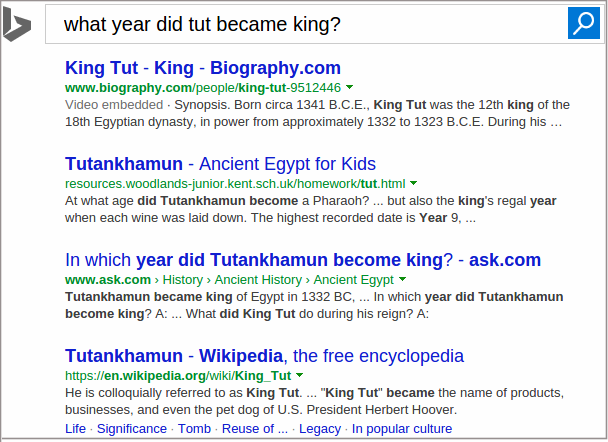
\includegraphics[width=0.5\textwidth]{img/web_search_entitylink}
\caption{Search results for the question ``what year did tut became king?''}
\label{fig:web_search_entitylink}
\end{figure}

The first problem that a KBQA system is facing is question entity identification.
The performance of the whole system greatly depends on this stage \cite{yao-scratch-qa-naacl2015}, because it seeds the answer candidate search process.
Question text is often quite short, may contain typos and other problems, that complicate question entity identification.
Existing approaches are usually based on dictionaries that contain entity names, aliases and some other phrases, which were used to refer to entities \cite{SPITKOVSKY12.266}.
These dictionaries are often noisy and incomplete, \eg to answer the question \textit{``what year did tut became king?''} a system needs to detect a mention \textit{``tut''}, which refers to the entity \textit{``Tutankhamun''}.
A mapping \textit{tut $\rightarrow$ ``Tutankhamun''} is missing in the dictionary used by one of the state of the art systems and therefore it couldn't answer this question correctly.
Instead of increasing the dictionary size we propose to use web search results to find variations of question entity names, which can be easier to link to a KB.
This idea was used for entity linking in web search queries \cite{SMAPH_ERD:2014}, which was given as one of the tracks on the Entity Recognition and Disambiguation Challenge 2014\footnote{http://web-ngram.research.microsoft.com/ERD2014/}.
Figure \ref{fig:web_search_entitylink} presents web search results for the query \textit{``what year did tut became king?''}, which shows that indeed many documents mention the full name, which can easily be mapped to a KB entity.

After question entities have been identified the next step is to explore their neighborhood and build structured queries as candidate answers.
A query addresses one or multiple KB predicates, which should be somehow related to words and phrases in the question and systems try score these mappings in order to select the best answer.
Existing knowledge base question answering approaches \cite{ACCU:2015,Berant:EMNLP13,berant2014semantic,berant2015imitation,BordesCW14:emnlp,yao2014freebase} rely on some kind of a lexicon, which is learned from manually labeled training data and supported by some additional resources, such as question paraphrases \cite{berant2014semantic} and weakly labeled sentences from a large text collection \cite{yao2014information}.
However, given the fact that manually labeled training data is very limited, such lexicons do not cover thousands of different predicates present in a KB.
By our estimate in a popular WebQuestions KBQA dataset answers to $\sim$5.5\% of test questions (112 out of 2032) involve a predicate, that doesn't appear in the training set.
For example, an RDF triple \texttt{[Bigos, food.dish.type\_of\_dish1, Stew]} answers a test question \textit{``what are bigos?''}, but there are no questions from the training set that are answered using the same predicate.
In addition, even if training set contains an example targeting a particular KB predicate, the lexicon might not cover all the other possible ways the same information can be asked about.
For example, test question \textit{``who is the woman that john edwards had an affair with?''} is similar in meaning and is answered with a similar query as a training set question \textit{``who did jon gosselin cheat with?''}, but the word \textit{affair} isn't used in the training set.
On the other hand, traditional text-based question answering systems benefit from the redundancy with which the same information is stated in many different ways in many documents \cite{Lin:2007:EPU:1229179.1229180}.
This increases the chances of a good lexical match between a question and answer statements, which makes even some relatively simple counting-based techniques quite effective \cite{brill2002analysis}.
We propose to borrow some ideas from text-based question answering and enrich the representation of candidate structured queries with additional text documents and fragments, that can help to select the best answer.
For example, the right part of the Figure \ref{fig:model} shows web search results, community question answering page and text fragments mentioning pairs of entities, that can clearly be useful to answer the question about John Edwards' affair.

\subsection{Contributions}

Our main contributions in this work are three-fold:
\begin{itemize}
\item a novel ``hybrid'' knowledge base question answering system, which uses both structured data from a knowledge base and unstructured natural language resources connected via entity links. Section \ref{section:method} describes the architecture of our system, and Section \ref{section:eval} shows that this fusion improves the performance of a state of the art KBQA system.
\item novel data sources for knowledge base question answering. Entity linking allows us to connect test resources with a KB. We explore three different types of text data, that is useful for KBQA: web search results (Section \ref{section:method:web}), Community Question Answering data (Section \ref{section:method:cqa}) and entity pairs language model based on a large text corpus (Section \ref{section:method:clueweb}).
\item evaluation and analysis. We evaluate the performance of our system on a popular WebQuestions dataset and demonstrate that using additional text resources we can improve the quality of knowledge base question answering (Section \ref{section:eval}). In addition, we conduct an extensive analysis of the system and suggest directions for future research (Section \ref{section:analysis}).
\end{itemize}

% -------------------------------------------

%There are many problems in KBQA:
%\begin{itemize}
%\item lexical variations, we can call the same thing in million ways
%\item representation variation - similar data can be represented in multiple ways, e.g. capital of the state in Australia location.australian\_state.capital\_city, while in the US you will have totally different predicate. HOWEVER, these are old predicate and marked deprecated. There is another predicate that should be the same for both cases.
%\item Incomplete, some data is simply missing or details are not present. E.g. who is the woman that john edwards had an affair with?, there is a triple that says that he had sexual relationships with Rielle Hunter, but there is no details...
%\item Related to the previous - many predicates are simply not present. There is something related, but not exactly what is asked about. Example: where did andy murray started playing tennis? We can find the answer entity, but the triple won't say that he started playing there.
%\end{itemize}

%In \cite{Sun:2015:ODQ:2736277.2741651} authors report pretty low score for Sempre on TREC and Bing QA datasets.

% Questions and corresponding answers are often expressed differently and researchers in question answering studied different ways to bridge this lexical gap, \eg using translation models \cite{Murdock:2005:TMS:1220575.1220661} and distributional semantics \cite{yu2014deep}.




\section{Problem}
\label{sec:problem}
\input{problem.inc}

\section{Models}
\label{sec:model}
\input{model.inc}

\section{Experiments}
\label{sec:experiments}
\input{experiments.inc}

\section{Error analysis and future work}
\label{sec:analysis}
% We have shown that Text2KB outperforms the baseline.
We now investigate how our system would compare to other systems on the same benchmark; then, we investigate in depth the different error modes (Section \ref{section:analysis:error}), which helps identify the areas of most substantial future improvements. 

\begin{table}
\centering
\caption{Average Recall (R), Precision (Pr), and F1 for Text2KB (our system), STAGG and their combinations}
\label{table:combine_stagg}
\begin{tabular}{| p{4cm} | p{1cm} | p{1cm} | p{1cm} | }
\hline
System & R & P & F1 \\
\hline
%Aqqu (baseline) \cite{ACCU:2015} & 0.604 & 0.498 & 0.494\\
% DIDN'T HAVE TIME TO IMPLEMENT THIS.
% Text-only baseline & & & & \\
Our system: Text2KB & 0.6354 & 0.5059 & 0.5223 \\
STAGG \cite{yih2015semantic} & 0.607 & 0.528 & 0.525\\
\hline
Text2KB + STAGG & 0.5976 & 0.5343 & 0.5320 \\
Text2KB + STAGG (oracle) & 0.7144 & 0.5904 & 0.6056 \\
\hline
\end{tabular}
\end{table}

We took an existing KBQA systems and demonstrated that by combining evidence from knowledge base and external text resources we can boost the performance.
A reasonable question is whether the same approach will be helpful to other systems, \eg the currently best system -- STAGG \cite{yih2015semantic}.
STAGG differs from our baseline system Aqqu in the components: entity linking algorithm, a set of query templates and ranking methods.
Therefore, our approach is complementary and should be helpful for STAGG as well.
To support this claim, we made an experiment to combine answers of STAGG and Text2KB.
One of the advantages of the former is its set of filters, that restricts list results to entities of certain type, gender, \etc
Therefore, we combined answers of STAGG and Text2KB using a simple heuristic: we chose to use the answer returned by STAGG if the number of answer entities is less than in the Text2KB answer, otherwise we use the answer of our approach.
Table \ref{table:combine_stagg} gives the results of the experiment, and as we can see the combination achieves slightly a better average F1 score.
Alternatively, we can look at the oracle combination of the systems, which always selects the answer with higher F1, which demonstrate that systems don't make exactly the same mistakes and therefore can be combined.
As we can see such a combination results in a performance of 0.6056, which is much higher than either of the systems.

As we mentioned earlier, answers to 112 of the test questions in WebQuestions dataset involve a predicate that weren't observed in the training set, which may be a problem for approaches that rely on a trained lexicon.
We evaluated both systems on these questions, and indeed the performance is very low, \ie the average F1 score of Text2KB is 0.1640 compared to 0.1199 for STAGG\footnote{Unfortunately, the number of questions is too low to show statistical significance (p-value=0.16)}.

\subsection{Error analysis}
\label{section:analysis:error}

\begin{figure}
\centering
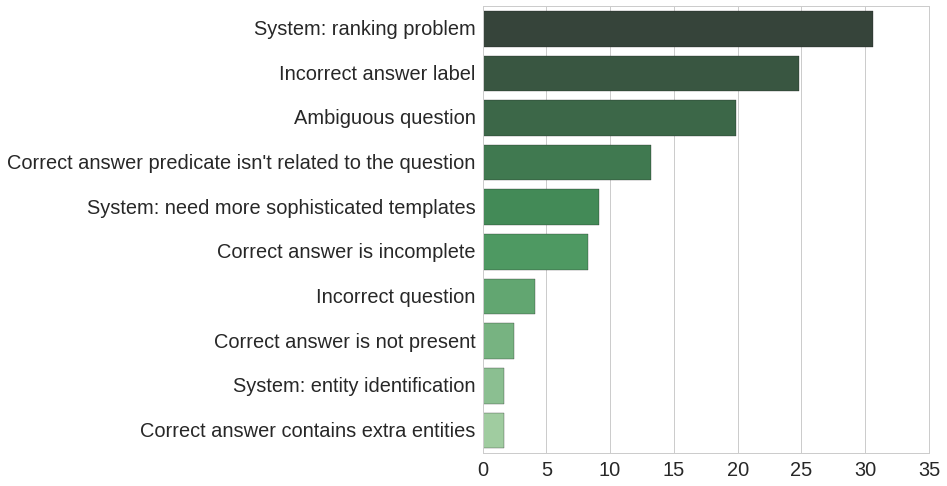
\includegraphics[width=0.45\textwidth]{img/error_analysis}
\vspace{-0.5cm}
\caption{Distribution of problems with questions, where Text2KB returns an answer with F1$<$1}
\label{fig:error_analysis}
\vspace{-0.3cm}
\end{figure}

To get a better insights into the problems that remain, we collected 1219 questions for which Text2KB didn't return completely correct answer, \ie F-1 score $<$ 1.
We manually looked through a couple of hundreds of these examples and grouped the problems into several clusters (Figure \ref{fig:error_analysis}).

As we can see candidate ranking is still the major problem, and it accounts for $~31\%$ of the cases.
The second most popular problem is incorrect ground truth labels (almost a quarter of errors).
For example: for the question \textit{when tupac was shot?''} the label says \texttt{Tupac 1994 assault} instead of \texttt{Las Vegas}.
Another set of questions have incomplete or overcomplete ground truth answer list.
Typical examples are questions asking for a list of movies, books, landmarks, \etc
The ground truth answer usually contains $\sim10$ entities, whereas the full list is often much larger.
This seems to be an artifact of the labeling process, where the answer was selected from the Freebase entity profile page, which shows only a sample of 10 entities, while the rest is hidden behind the ``NNN values total'' link.
About 20\% of the questions are ambiguous, \ie questions have no strict 1-1 correspondence with any of the predicates and can be answered by multiple ones without any obvious preferences.
% for the question \textit{``where is shakira from?''} the ground truth is the country - \texttt{Colombia}, while Text2KB returned her place of birth - \texttt{Barranquilla}.
For example, the question \textit{``what did hayes do?''} can be answered by profession, occupied position or some other achievements.
Another problem is when there is no predicate that answers the question.
For example, the question \textit{``what do people in france like to do for fun?''} doesn't have a good match among the facts stored in Freebase.
The ground truth entity \texttt{Cycling} comes from the list Olympic sport competitions country participated\footnote{\texttt{olympics.olympic\_participating\_country.athletes}}.
% In some cases there are entities that are very similar in meaning, but represented in Freebase by different ids and names.
% For example, the answer to the question \textit{``what is william taft famous for?''} is \textit{``President of the United States''}, which is a government position, but there is also a triple \texttt{[William Howard Taft, common.topic.notable\_for, US President]}, where the last entity represents a type of people who help the position, and is considered incorrect.

% This is nice, but probably is too little to mention.
% We also noticed, that in a small number of examples, the case of the correct answer entity and the answer returned by the system is different.
% For example, for the question \textit{``what fma stands for?''} the correct answer specified in the dataset is \textit{``FullMetal Alchemist''}, while the actual name of the entity is \textit{``Fullmetal Alchemist''}.
% The official evaluation script don't normalize the case and therefore considers this example incorrect.
% If we lowercase all entity names before comparison, the average F1 score of Text2KB becomes 0.5248.

Text2KB components were quite effective in resolving some of the problems.
Web search results helped identify the right question topical entity in a number of cases, \eg \textit{``what did romo do?''} mentions only the last name of the Dallas Cowboys quarterback and the baseline system were unable to map it to the right entity.
Web search results provides more than enough evidence that romo refers to \texttt{Tomo Romo}.
However, there are a number of loses, introduced by added unrelated entities.
For example, the entity \texttt{I Love Lucy} was added for the question \textit{``what was lucille ball?''}, because the term \textit{lucy} had high similarity with \textit{lucille}.
A portion of these problems can be fixed by a better entity linking strategy, \eg \cite{SMAPH_ERD:2014}.
An interesting example, when external text resources improved the performance is the question \textit{``what ship did darwin sail around the world?''}.
This is actually a hard question, because the ship entity is connected to the \texttt{Charles Darwin} entity through the ``knownFor'' predicate along with some other entities like \texttt{Natural selection}.
% \footnote{\texttt{user.lindenb.default\_domain.scientist.known\_for}
Thus, the predicate itself isn't related to the question, but nevertheless, the name of the ship \texttt{HMS Beagle} is mentioned multiple times in the web search results, and entity pair model computed from ClueWeb also has high scores for the terms ``ship'' and ``world''.

There are several major reasons for the loses, introduced by features based on external text resources.
Some entities often mentioned together and therefore one of them gets high values of cooccurrence features.
For example, the baseline system answered the question \textit{``when did tony romo got drafted?''} correctly, but since \texttt{Tony Romo} is often followed by \texttt{Dallas Cowboys}, Text2KB ranked the team name higher.
Another common problem with our features is an artifact of entity linking, which works better for names and often skips abstract entities, like professions.
For example, the correct answer to the question \textit{``what did jesse owens won?''} is an entity with the name \texttt{Associated Press Male Athlete of the Year}, which is rarely mentioned or it's hard to find such mentions.
Some problems were introduced by a combination of components.
For example, for \textit{``where buddha come from?''} a topical entity \texttt{Buddhism} was introduced from search results, and it generated \texttt{Gautama Buddha} as one of the answer candidates.
This answer was ranked the highest due to large number of mentions in the search results.

In summary, we show that ideas behind Text2KB could be integrated into other systems and improve their performance.
The error analysis suggested that even though a significant number of questions in the WebQuestions dataset have incorrect or ambiguous ground truth labels, there is still a room for improvement.
In particular, the future work for Text2KB will include a better strategy for entity linking using external data sources and a better context model for entity mentions in text documents, which can put more weight on entities mentioned in the context related to the question.


\section{Related work}
\label{sec:relatedwork}

Recent development of large scale knowledge bases (e.g. dbPedia \cite{auer2007dbpedia}) and Freebase \cite{Bollacker:2008:FCC:1376616.1376746}) motivated research in open domain question answering over linked data.

In 2011 a series of QALD (Question Answering over Linked Data) evaluation campaigns has started, report on the last one, QALD-5, can be found in \cite{UngerFLNCCW15}.
These benchmarks target dbPedia as a knowledge base and provide a rather small (50-350) training set of questions, annotated with correct SPARQL queries.
In QALD-3 a multilingual task has been introduced, and since QALD-4 it includes the hybrid task, that asks participants to build systems that can use both structured data and free form text available in dbPedia abstracts.
The formulation of the hybrid task is the most relevant to our work, however, there are a couple of key differences: unlike this work the hybrid task questions are manually created so that they could \emph{only} be answered by combining RDF and text data.
The second difference lies in the nature of text data used for question answering.
In this work we use a broad spectrum of various text resources, such as web search results, CQA archives and semantically enriched text documents, while the focus of the task is on relatively short abstracts.
Lastly, because of the expensive labeling process QALD datasets are small, for example, QALD-5 training set for multilingual question answering included 300 examples and hybrid - 40 examples (the evaluation was done on 50 questions for multilingual task and just 10 for hybrid).
The scale of the datasets makes it hard to use machine learning, which lies in the heart of this work.
For these reasons, we didn't include QALD in our evaluation experiments.
However, we acknowledge the importance of QALD and intend to look into it and especially into the hybrid track in the future.

WebQuestions benchmark dataset was developed in \cite{Berant:EMNLP13} and since triggered a number of works that explored both semantic parsing and information extraction approaches for KBQA \cite{yao2014freebase}.
Developed system differ in ways question entity is detected, candidate answers are generated, features used and the answer is selected.
The most interesting aspect for this work is the use of external resources, that help translate natural language text into KB properties and entities.
Such a lexicon can be learned from a labeled training set \cite{Berant:EMNLP13},  ClueWeb collection aligned to Freebase \cite{yao2014information}, question paraphrases clusters from WikiAnswers \cite{berant2014semantic}, Freebase triples rephrased as questions \cite{BordesCW14:emnlp}, and can be based on the embeddings of questions and knowledge base entities and predicates \cite{BordesCW14:emnlp,yih2015semantic}.
However, most of the models are still biased towards the types of questions present in the training set and would benefit from more training data.
In this work I propose to extend the training set with question-answer pairs available on CQA websites, which were shown to be useful for relation extraction \cite{savenkov-EtAl:2015:SRW}.
In addition, I propose to use unlabeled text resources for candidate query ranking, which can help to generalize to unseen types of questions and questions about predicates never mentioned in the training set.

In general, combination of different data sources, such as text documents and knowledge bases, for question answering is not a novel idea and it has been already implemented in hybrid QA systems \cite{baudivs2015modeling}, \eg IBM! Watson combined text and structured data resources in their Jeopardy! winning system \cite{Barker12}.
The key difference of our approach is that such hybrid systems typically have separate pipelines to generate candidate answers from different data sources and only rank them together to select the best one.
In this work we attempt to integrate text resources inside the KBQA answer generation and scoring.

Another interesting attempt to combine the data sources has been made by  \cite{Sun:2015:ODQ:2736277.2741651}, who showed that entity types and descriptions can be effectively used by text-based question answering systems.
In this work, we focus on the inverse problem of improving knowledge base question answering by incorporating natural language text resources.
..... MENTION JEFF DALTON'S WORK ON ENTITY ENRICHMENT \cite{dalton2014entity}.

Open IE extractions \cite{fader2011identifying} represent an interesting mixture between text and structured data and can be considered as an intermediate step between raw text and structured KB.
Such knowledge repositories can be queried using structured query languages such as SPARQL and at the same time allows text matching against entities as predicates.
One can easily transform an existing KB to such a form by replacing predicates and entities with their names and  \cite{Fader:2014:OQA:2623330.2623677} demonstrated that even though such an approach looses to existing baselines on WebQuestions dataset, where questions are known to be answerable from KB, achieves higher scores on TREC and WikiAnswers benchmarks.


\section{Conclusion}
\label{sec:conclusion}
\input{conclusion.inc}

\vspace{-1mm}
\section*{Acknowledgments}
\vspace{-1mm}
This work was funded by the Google Faculty Research Award.
We gratefully thank Evgeniy Gabrilovich and Amar Subramanya for numerous valuable and insightful discussions, and anonymous reviewers for useful comments on the work.

\bibliography{biblio}
\bibliographystyle{naaclhlt2015}

\end{document}
